\section{Exercise and Report}
\subsection{Voltage Follower}
Voltage follower is one of the simplest uses of an operational amplifier, where the output
voltage is exactly same as the input voltage applied to the circuit. In other words, the gain
of a voltage follower circuit is unity. The connections are proposed as follows:
\begin{figure}[h]
    \centering
    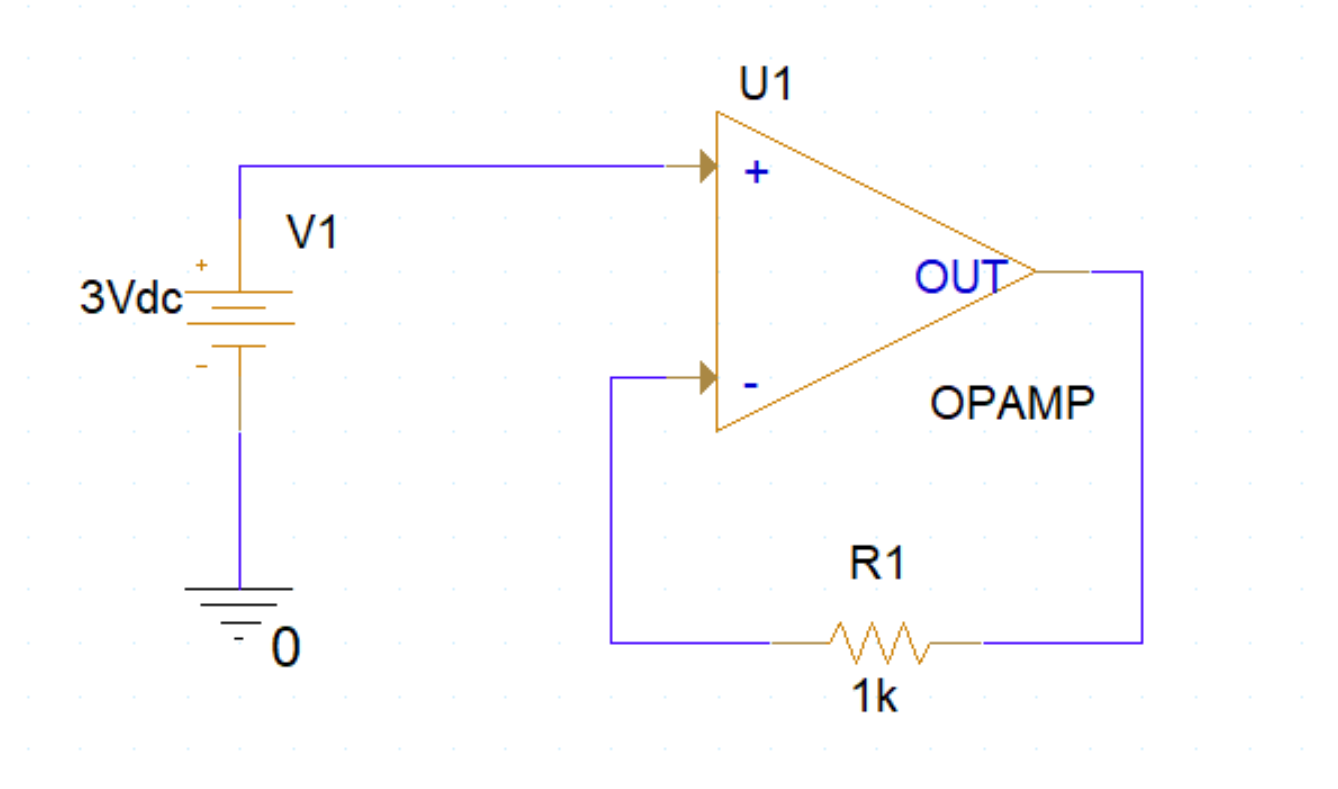
\includegraphics[width=0.6\textwidth]{graphics/ex1/f1.png}
    \caption{ Opamp follower circuit}
\end{figure}

A voltage follower has low output impedance and extremely high input impedance, and
this makes it a simple and effective solution to problematic impedance relationships.

If
a high-output-impedance sub-circuit must transfer a signal to a low-input-impedance
sub-circuit, a voltage follower placed between these two sub-circuits will ensure that the
full voltage is delivered to the load.

\textbf{Ảnh mô phỏng}

\begin{figure}[ht]
    \centering
    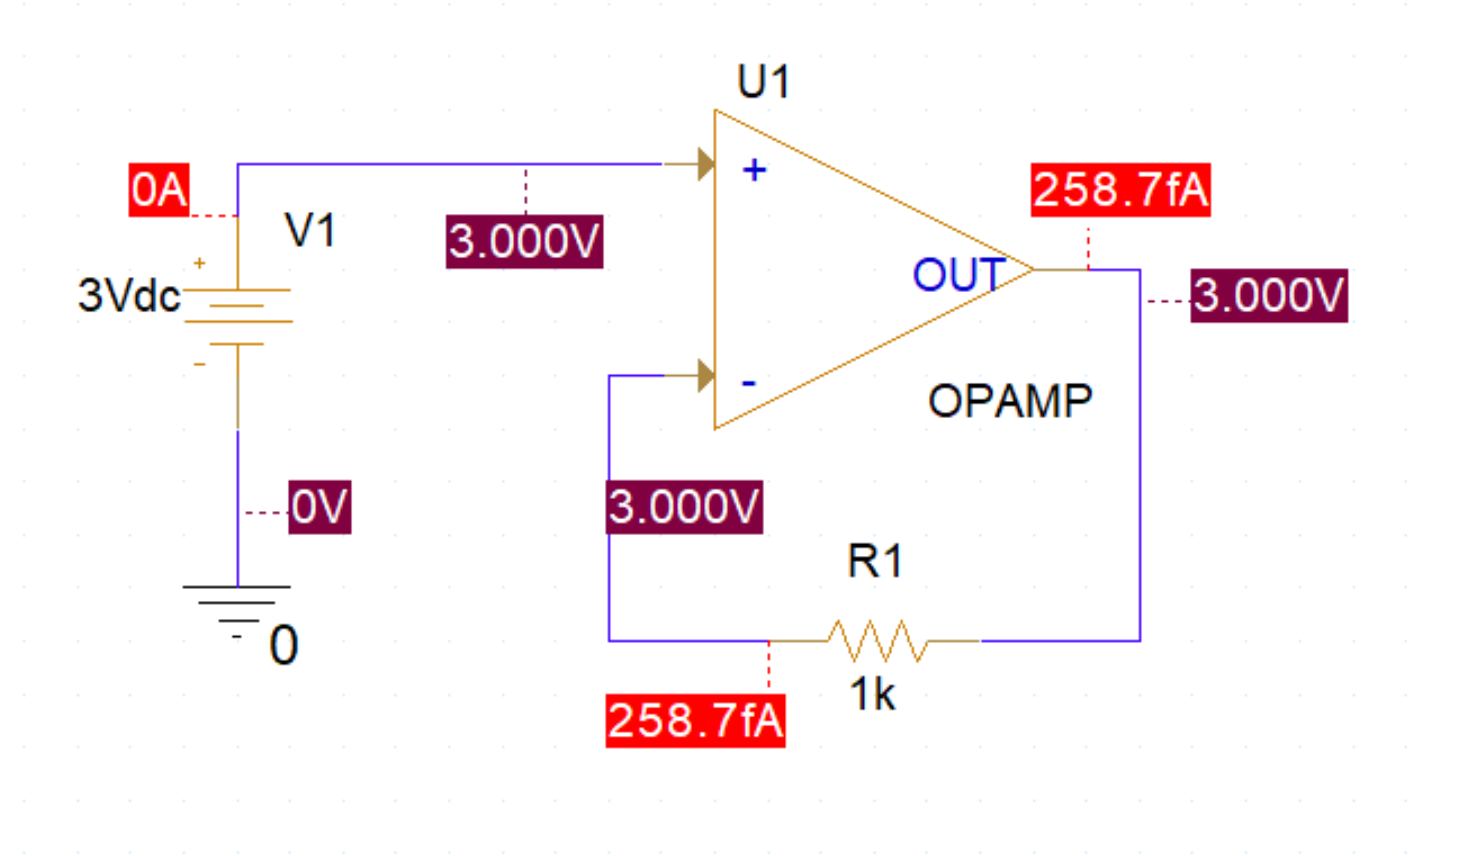
\includegraphics[width=0.6\textwidth]{graphics/ex1/f2.png}
    \caption{Simulation Opamp follower circuit with $R_1 = 1k \Omega$ }
\end{figure}

\begin{figure}[ht]
    \centering
    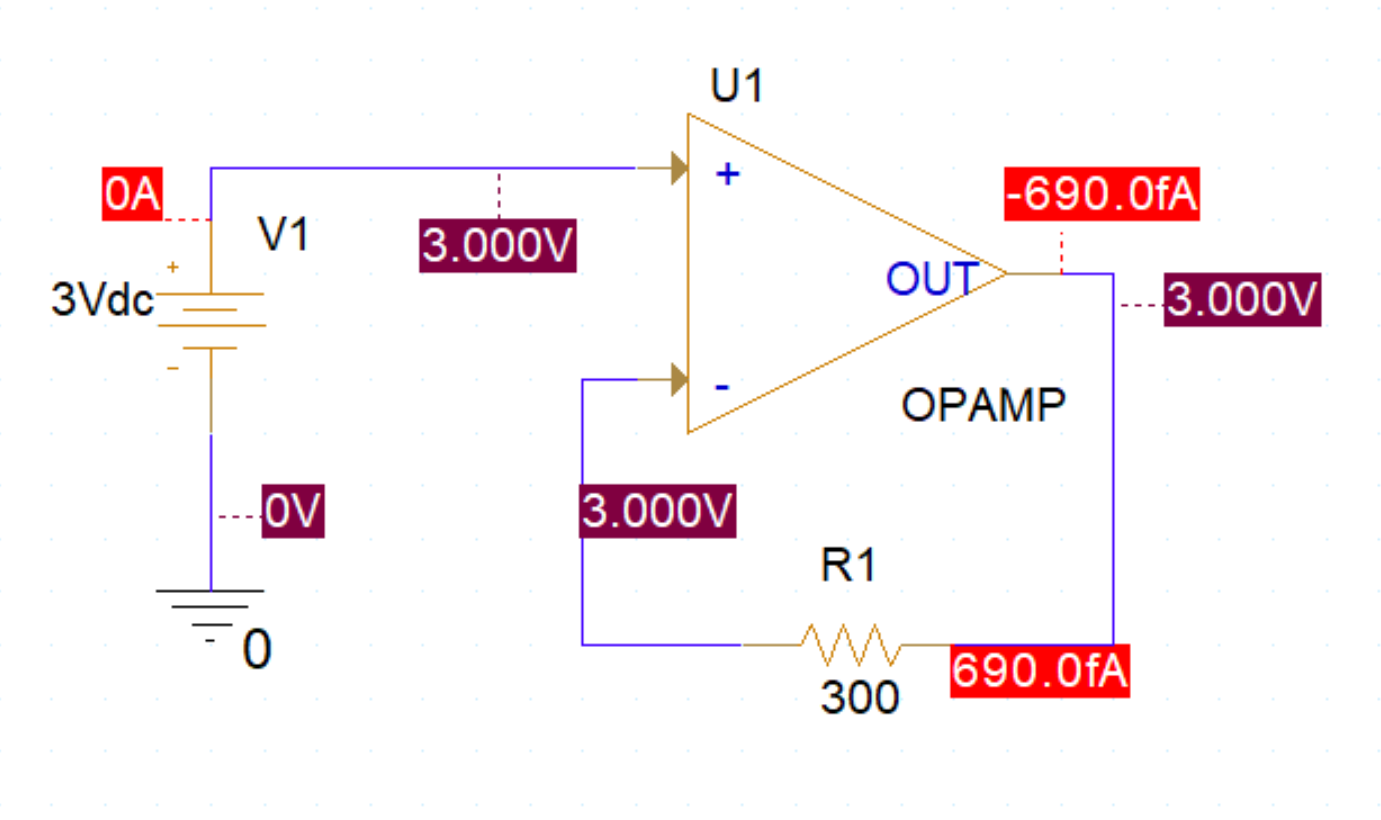
\includegraphics[width=0.6\textwidth]{graphics/ex1/f3.png}
    \caption{Simulation Opamp follower circuit with $R_1 = 300 \Omega$}
\end{figure}

Ta có mạch tương đương của Opamp như sau:

\begin{figure}[ht]
    \centering
    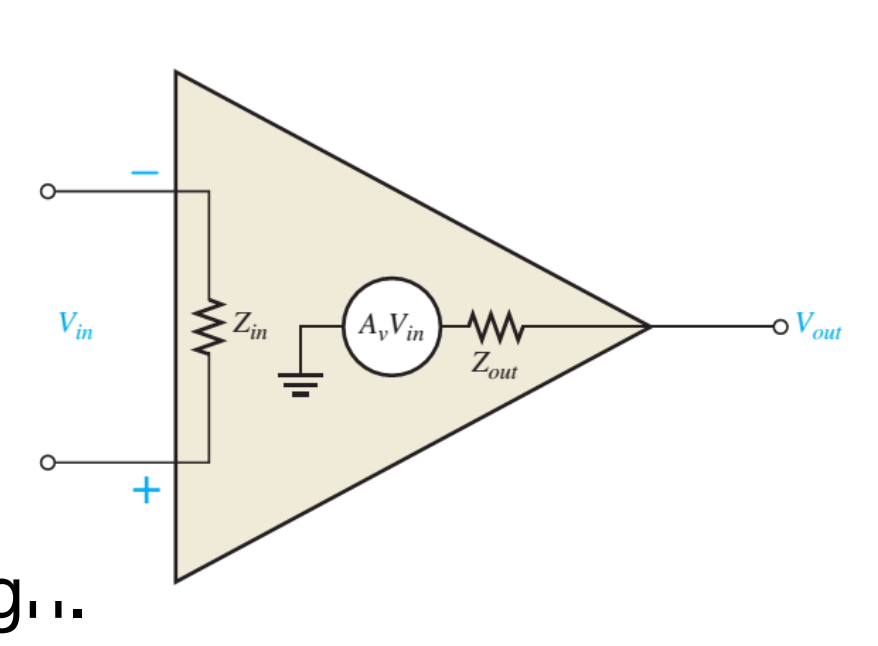
\includegraphics[width=0.6\textwidth]{graphics/ex1/f4.png}
    \caption{Mô hình thực tế của Opamp}
\end{figure}

Theo định luật Ohm, ta có: $I = \dfrac{V_{out} - V^+}{R_1 + Z_{in}}$

Mà trở kháng đầu vào ($Z_{in}$) rất lớn nên $I \approx 0$. Do vậy $V_{out} \approx V^+$ với bất cứ giá trị nào của $R_1$.
\pagebreak
\subsection{High-Current Voltage Follower}
The voltage follower's low output impedance makes it a good circuit for driving current
into a low-impedance load, but it's important to remember that most op-amps are not
designed to deliver large output currents. The most basic circuit for buffering an op-amp's
output current is the following:

\begin{figure}[ht]
    \centering
    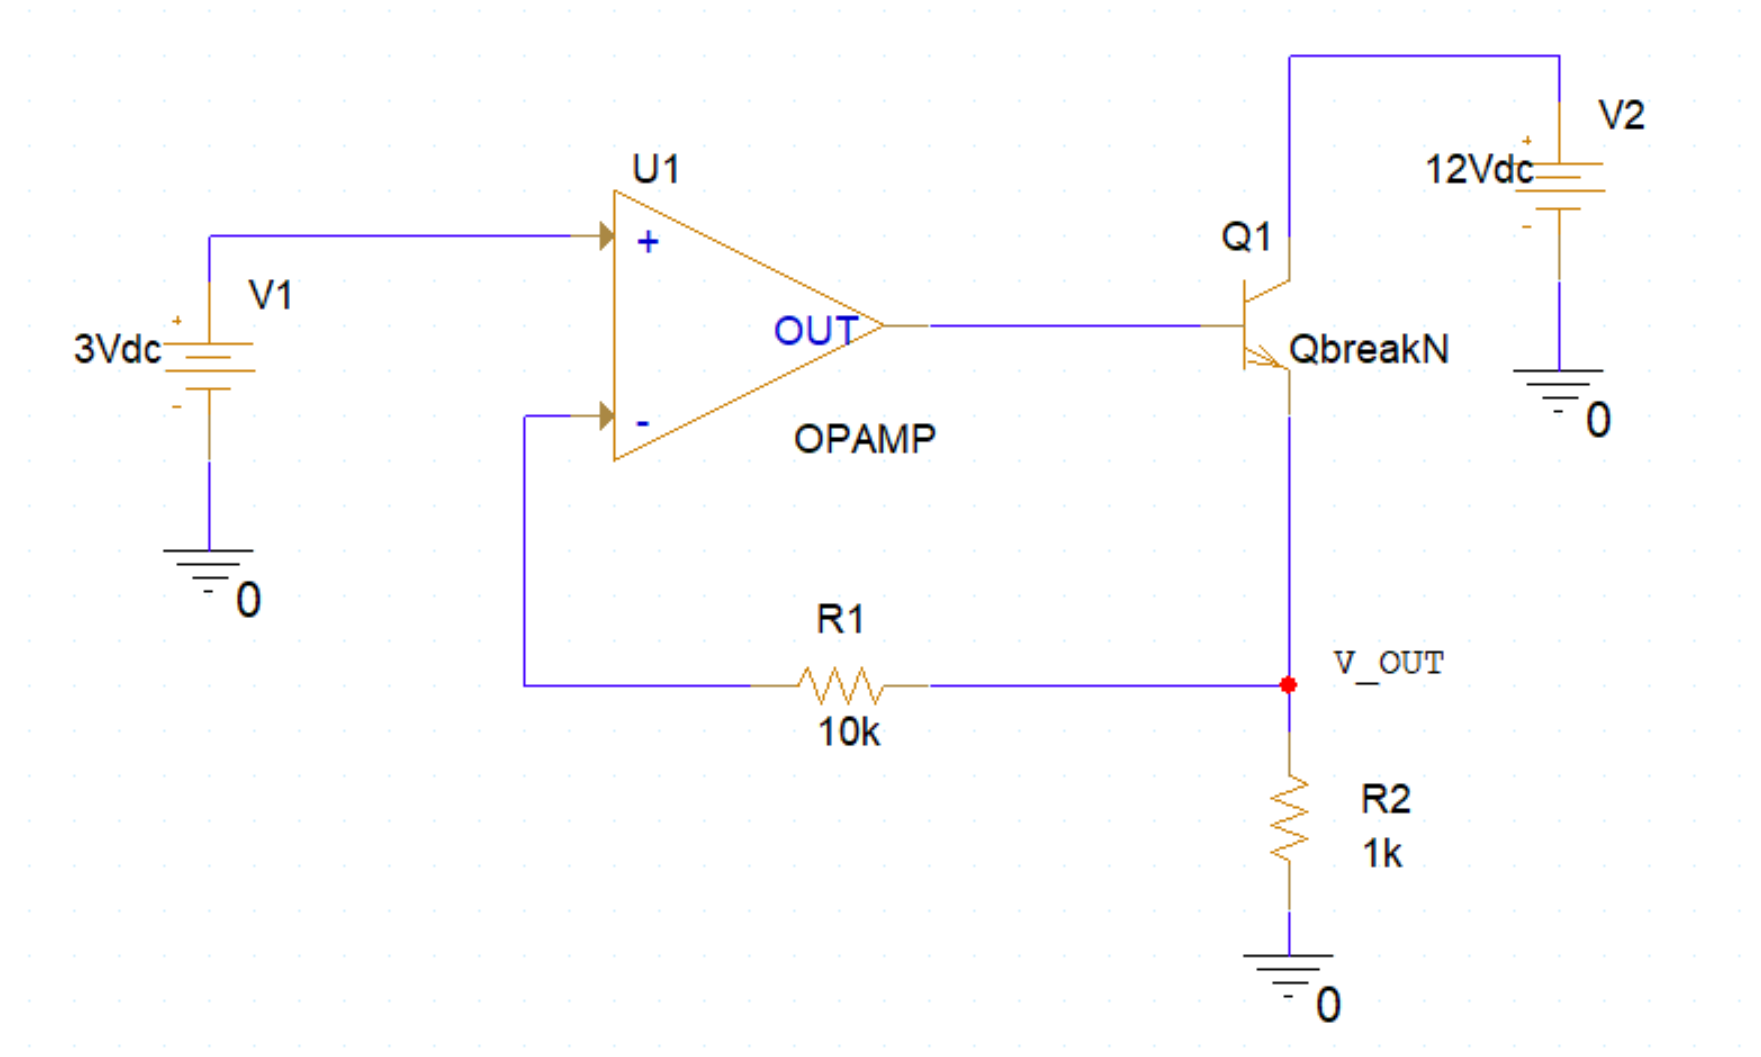
\includegraphics[width=0.8\textwidth]{graphics/ex1/f6.png}
    \caption{Opamp follower circuit}
\end{figure}

The voltage at the positive pin of the Opamp is copied to VOUT . In this schematic, R2 is
used to simulate a load device, which can be a motor or an high power LED. However, in
this case, there is a high current can pass the load.

\textbf{Ảnh mô phỏng}

\begin{figure}[ht]
    \centering
    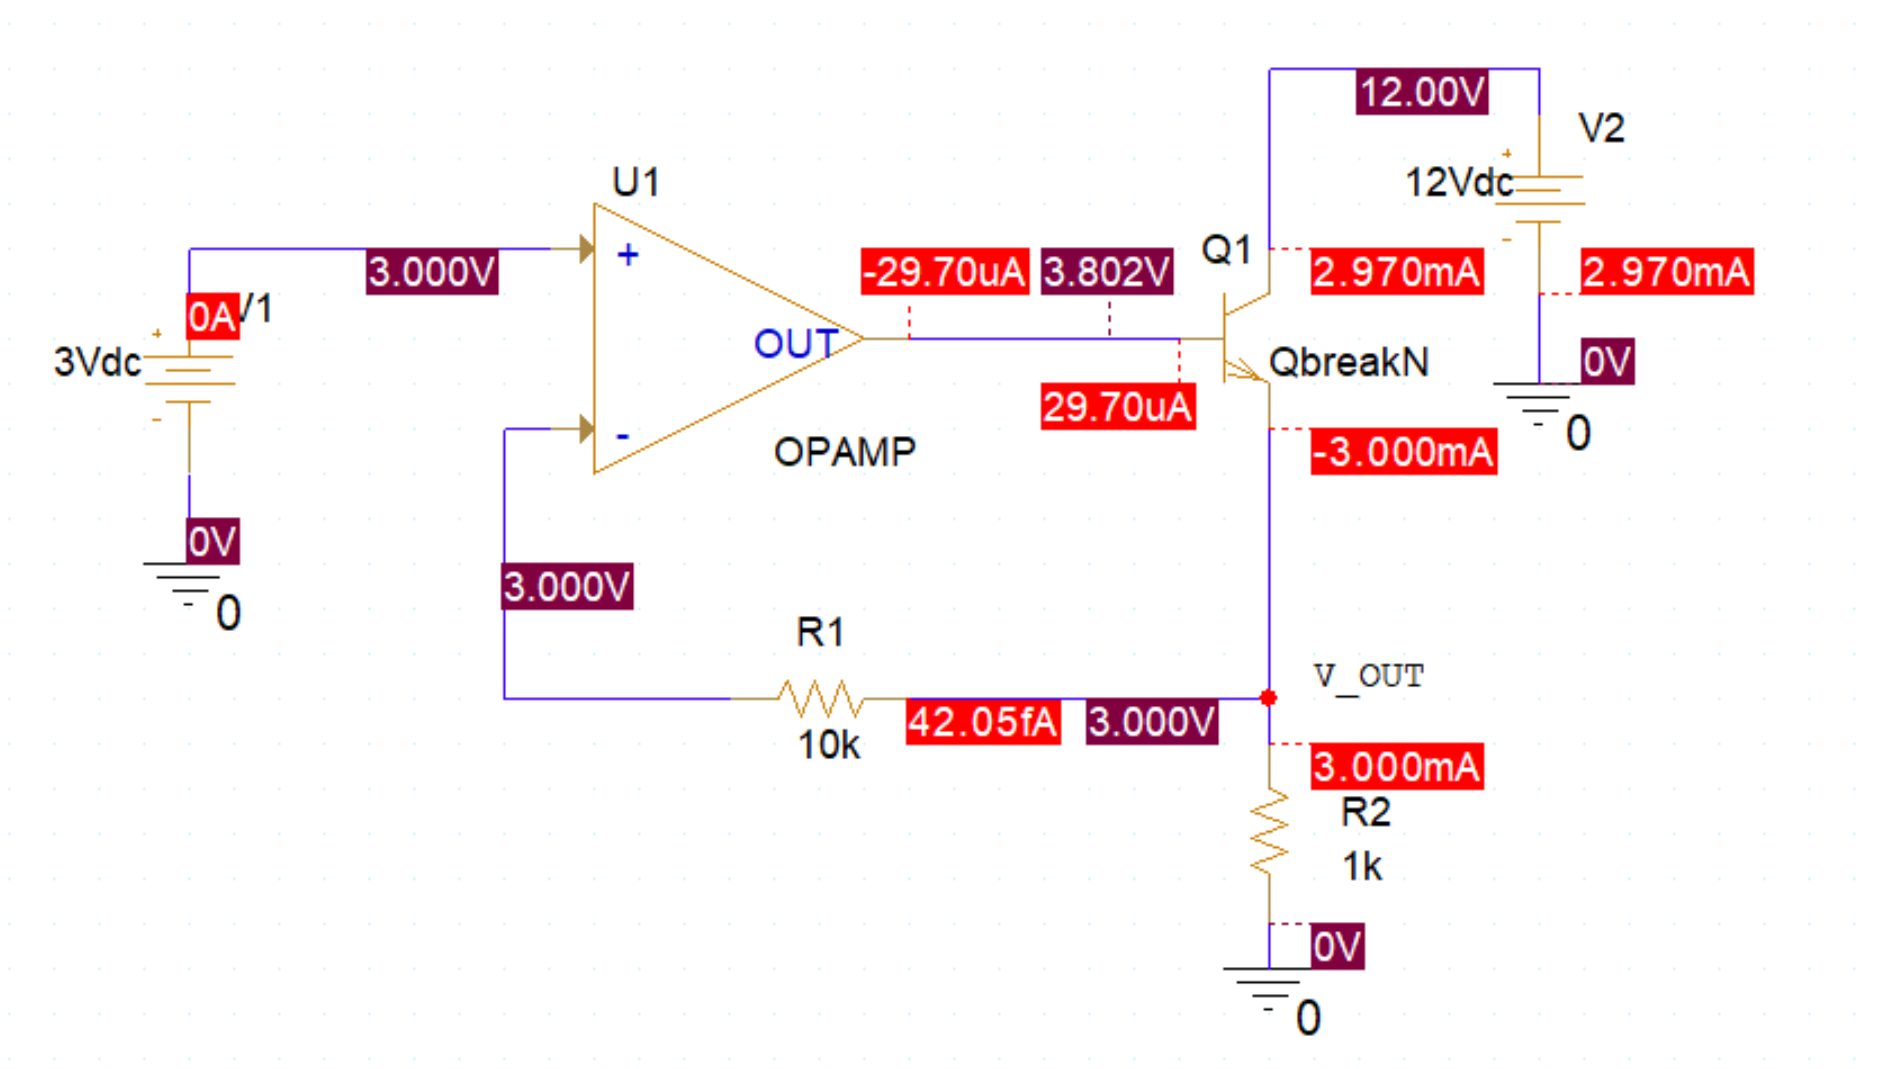
\includegraphics[width=1\textwidth]{graphics/ex1/f5.png}
    \caption{Simulation Opamp follower circuit}
\end{figure}
\pagebreak

Theo định luật Ohm, ta có: $I_{R_1} = \dfrac{V_{out} - V^+}{R_1 + Z_{in}}$

Mà trở kháng đầu vào ($Z_{in}$) rất lớn nên $I_{R_1} \approx 0$. Do vậy $V_{out} \approx V^+$ với bất cứ giá trị nào của $R_1$.

Với $V_{out} = V^+ = 3 V$, theo định luật Ohm: $I_{R_2} = \dfrac{V_{out}-0}{R_2} = 3 $ (mA).

Giả sử BJT ở vùng tích cực, $V_{BE} \approx 0.7$ V (Trong mô phỏng trên PSpice $V_{BE} \approx 0.8$ V) và $I_B = \beta I_C$ (Trong mô phỏng PSpice $\beta = 100$)

Do vậy, điện áp tại đầu ra của Opamp: $V_{Opamp\_out} = V_{BE} + V_{out} = 0.8 + 3 = 3.8 $ V và

$I_{R_2} = I_B + I_C = (1 + \beta)I_B = 101I_B \rightarrow I_B = \frac{I_{R_2}}{101} = 29.7(\mu A)$ và $I_C = 100I_B = 2.97$ (mA).
\pagebreak
\subsection{Voltage Follower with Gain}
This basic circuit is not limited to the unity-gain configuration. As with a non-buffered
op-amp, you can insert resistors into the feedback path to create overall gain from the
input to the load voltage. Here is the non-unity-gain version of the circuit:
Students are proposed to implement this circuit on PSPICE with input is 2V and the gain
is 3. The voltage supply for the load side is 12VDC. Value of RLOAD is 1K.

\begin{figure}[ht]
    \centering
    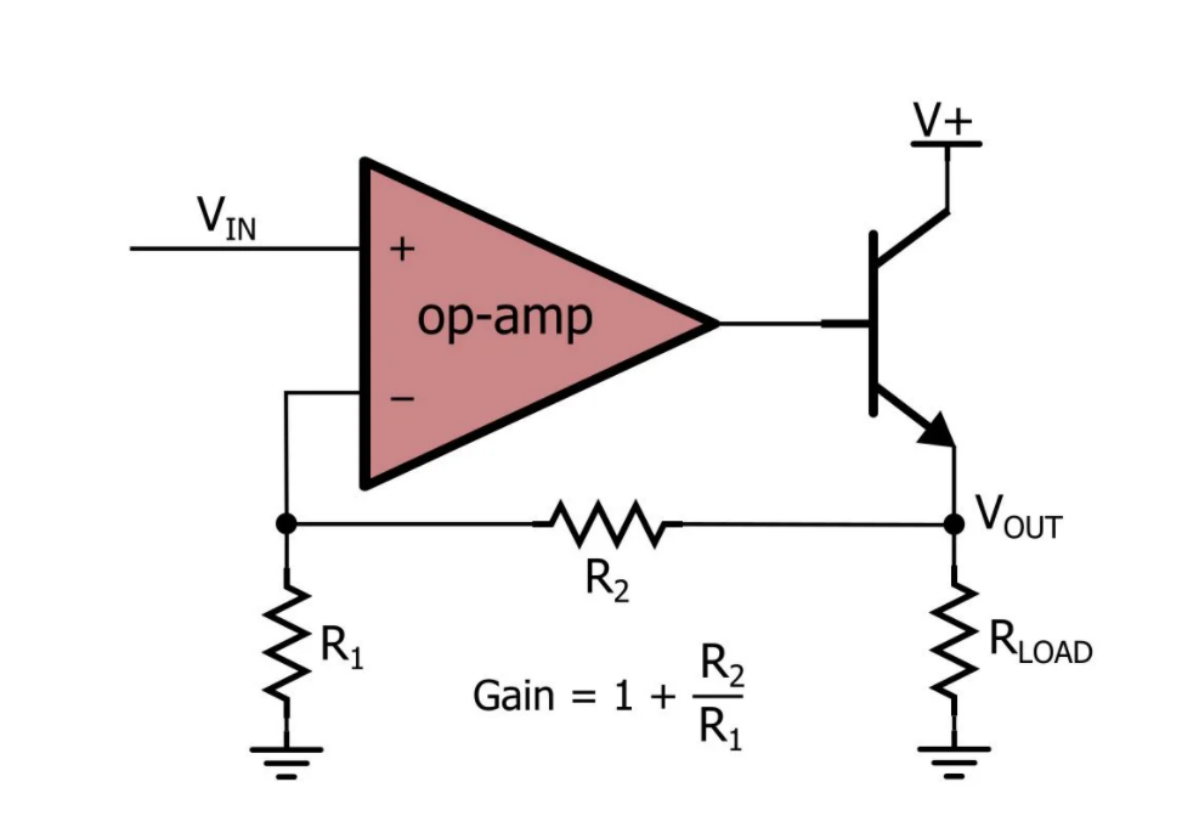
\includegraphics[width=0.5\textwidth]{graphics/ex1/f7.png}
    \caption{Opamp follower with gain for the output}
\end{figure}

\textbf{Ảnh mô phỏng}

\begin{figure}[ht]
    \centering
    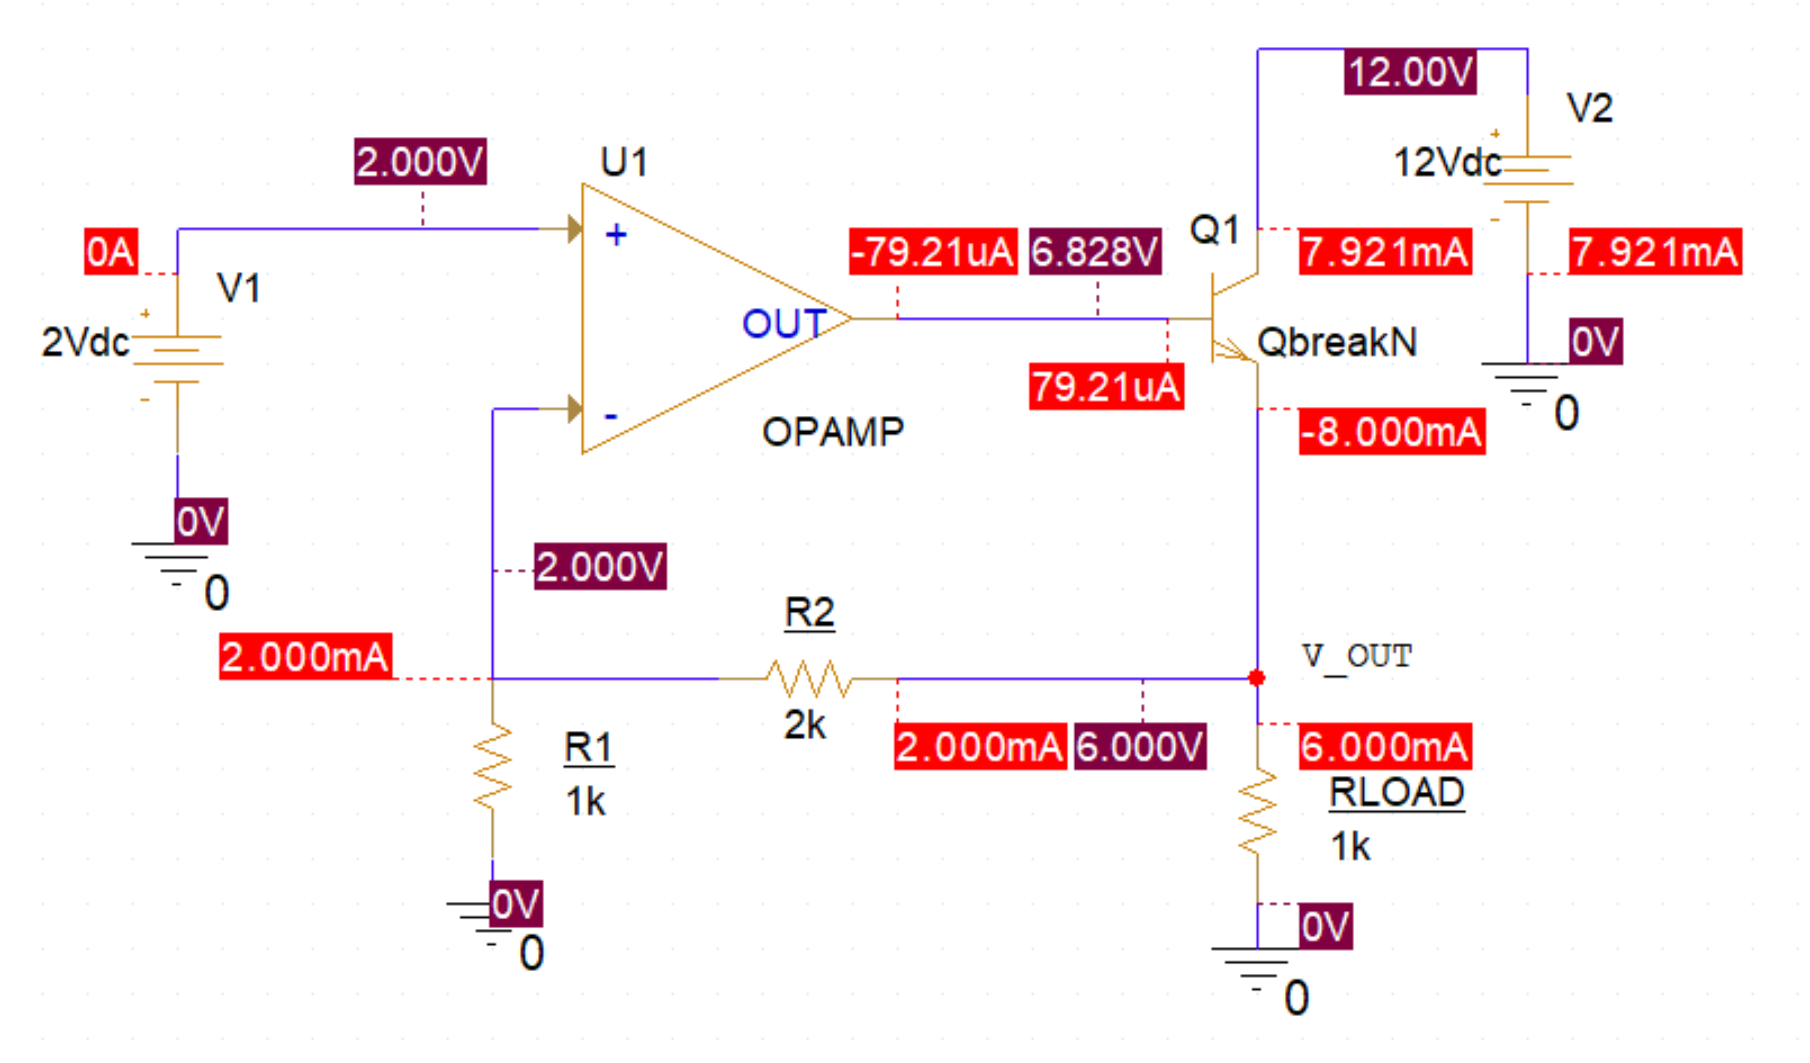
\includegraphics[width=0.95\textwidth]{graphics/ex1/f8.png}
    \caption{Opamp follower with gain for the output}
\end{figure}

Ta có, Opamp hồi tiếp âm do điện trở đầu vào lớn nên $V^+ = V^- = 2$ V

Mà $I_{Opamp^-} \approx 0$ nên $I_{R_1} = I_{R_2} = \dfrac{V^- - 0}{R_1} = \dfrac{V^+}{R_1}$

Theo định luật Ohm,  $I_{R_2} = \dfrac{V_{out} - V^-}{R_2} \rightarrow V_{out} = V^- + I_{R_2}R_2 = V^+ + \dfrac{V^+R_2}{R_1} = V^+(1 + \dfrac{R_2}{R_1})$

Hay $V_{out} = (1 + \dfrac{R_2}{R_1})V_{in} \rightarrow GAIN = \dfrac{V_{out}}{V_{in}} = 1 + \dfrac{R_2}{R_1}$.

Trong mô phỏng lấy ví dụ $R_1 = 1k$ và $R_2 = 2k$ để được GAIN = 3. Như vậy, ta có $V_{out} = 2.3 = 6$ (V).

Theo định luật Ohm, $I_{R_{LOAD}} = \dfrac{V_{out}}{R_{LOAD}} = \dfrac{6}{1k} = 6 $ (mA).

$V_{OPAMP\_out} = V_{BE} + V_{out} = 6 + 0,8 = 6,8$ (Trong mô phỏng lấy $V_{BE} \approx 0.8$ V) và

$I_{out} = I_{R_2} + I_{R_{LOAD}} = \frac{V_{in}}{R_1} + 6$ = 8 (mA)

$I_{out} = (1+\beta)I_B  = 101I_B \rightarrow I_B = 79,2 (\mu A) \rightarrow I_C = 100I_B = 7,92$ (mA) (Trong mô phỏng $\beta$ của BJT = 100)
\pagebreak
\subsection{Summing Amplifier}
Students are proposed to implement following schematic in PSPICE and run the simulation with R1 = 1K, R2 = 2K, R3 = 5K, Rf = 9K, Ri = 1K. There inputs are V1 = 1V, V2 = 2V and
V3 = 3V. This circuit is a non inverting summing configuration using opamp.

\begin{figure}[ht]
    \centering
    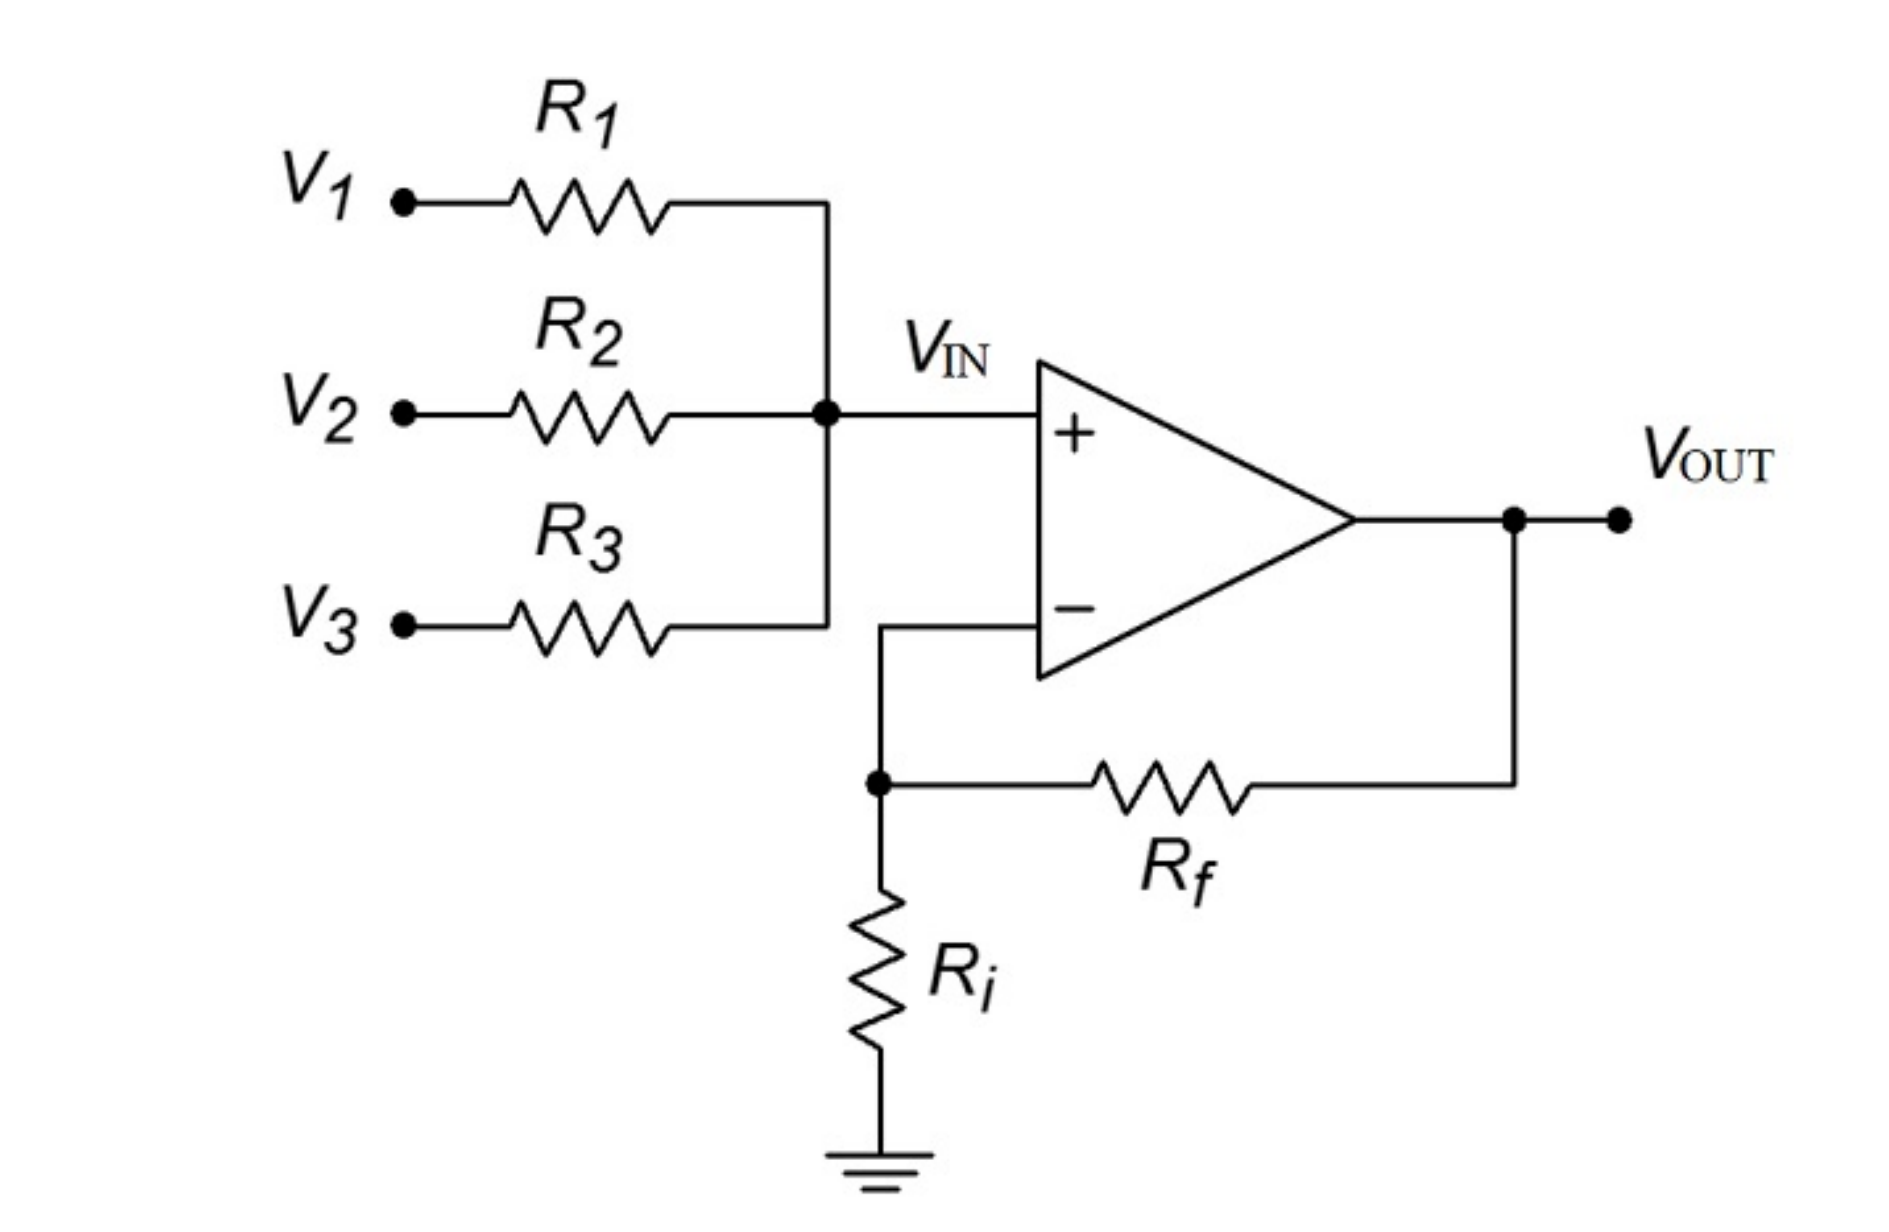
\includegraphics[width=0.7\textwidth]{graphics/ex1/f9.png}
    \caption{Non inverse summing using OPAMP}
\end{figure}

\textbf{Ảnh mô phỏng}

\begin{figure}[ht]
    \centering
    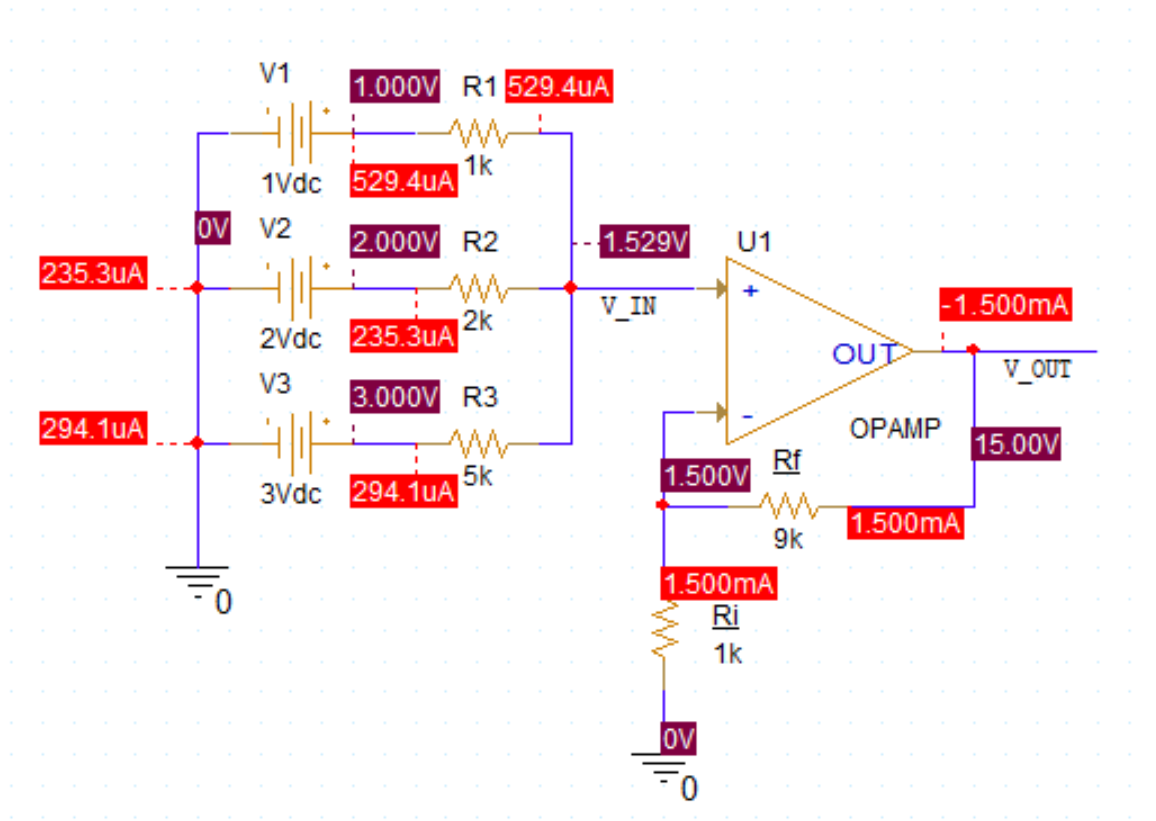
\includegraphics[width=1\textwidth]{graphics/ex1/f11.png}
    \caption{Non inverse summing using OPAMP}
\end{figure}

\pagebreak
\subsection{Low Pass Filter}
\subsection{High Pass Filter}
\subsection{Comparator with Hysteresis (Schmitt Trigger)}